\section{Assignment 6}
\subsection{Feature selection}
The first subtask of assignment six was to choose several quantitative  features, which are responsible for the same aspect.
This is not easy task when using our dataset because all our features are very heterogeneous.
So we did the best we could do: we have choosen features that in our opinion reflect attitude of the readers to the article: \texttt{num\_imgs},\texttt{global\_sentiment\_polarity},  \texttt{shares}. 
The meaning of such features are respectively as follows: number of images that are present in the article, expressivity of an article, number of shares in social media of that article. 
Some of this features (as was already described in previous homeworks) were substituted with it's logarithm  to get rid of lognormal distributions.

\subsection{Visualization with PCA}
To visualize features mentioned above on the 2D plane we first apply normalization of the data according to one of the following schemes: 
\begin{itemize}
	\item shift with midrange and rescale with half-range (aka \emph{range} standardization)
	\item shift with mean and rescale with standart deviation  (aka \emph{z-score} standardization)
\end{itemize}

Next we have applied conventional PCA for the data after it's standardization. 
The results of such standardization and subsequent PCA are shown in the Figure \ref{fig:PCA_hw6}.

\begin{figure}[h]
\hspace{-1cm}
\begin{minipage}[h]{0.49\linewidth}
\center{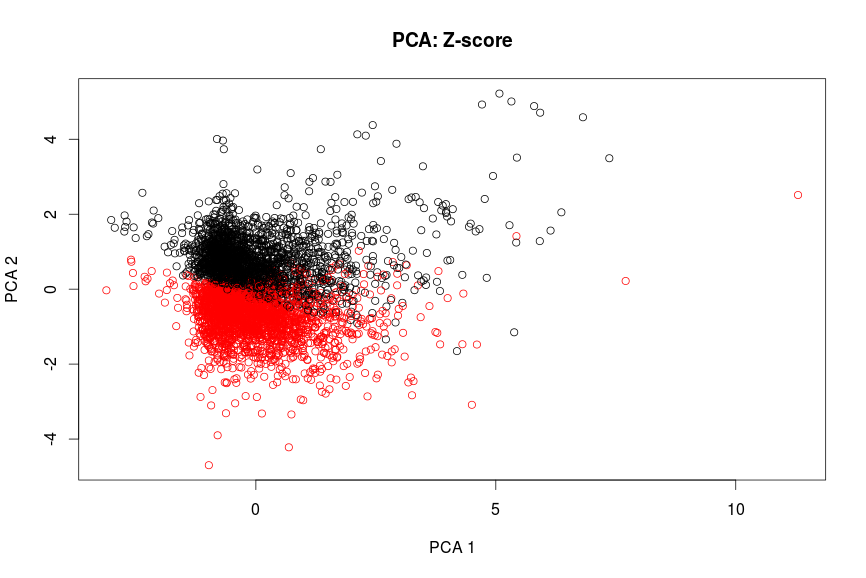
\includegraphics[width=1.1\linewidth]{PCA_zscore_hw6.png} \\ a)}
\end{minipage}
\hfill
\begin{minipage}[h]{0.49\linewidth}
\center{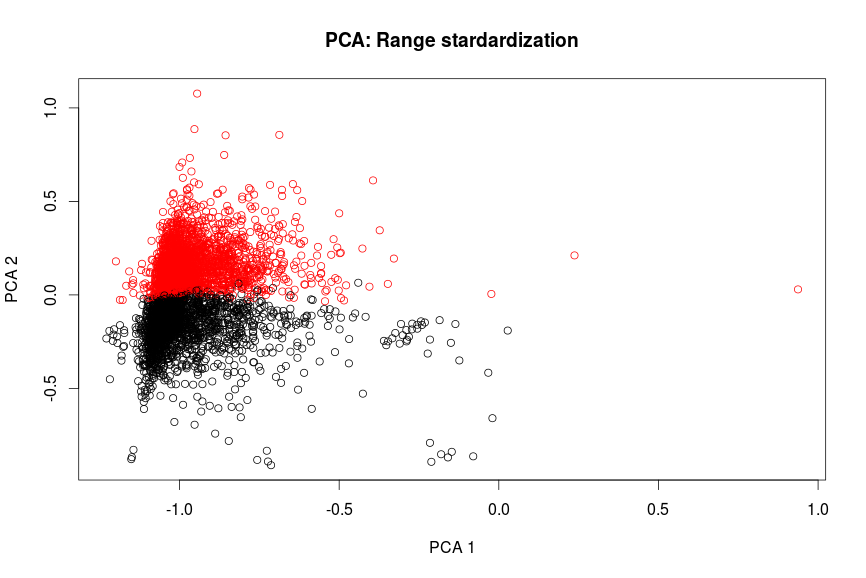
\includegraphics[width=1.1\linewidth]{PCA_rangenorm_hw6.png} \\ b)}
\end{minipage}
\caption{Scatter plots of 3D-data (\texttt{num\_imgs}, \texttt{global\_sentiment\_polarity},  \texttt{shares}) with different standardixation: z-scoring (a) and range standardization (b). Entities, responsible for articles with positive or negative overtones are marked as red and black points respectively.}
\label{fig:PCA_hw6}
\end{figure}

In this Figure one can see red and black circles which represent negative and positive mood of article respectively. Such a partition was explained in great detail in the previous assignment. 

One could also note, that z-score standardized data is not linearly separable. This is not the case for range standardization: in the b) figure one can see almost perfect linear separability. 

This could be explained with the type of distrubution of the data. According to the Shapiro-Wilks normality test chosen features are not normally distributed with the p-value almost zero. And according to \cite{CCODA_Mirkin} the less data distribution resembles normal the less one could hope to get interpretable results of analysis. 

One of the most interesing fact in this assignment is that the type of normalization strongly influence distribuion of contribution of principal components to the total data scatter. This is detailly explained in \cite{CCODA_Mirkin} and the additional evidence could be gained from the Figure \ref{fig:data_scatter_contibution}. 

So in further analysis and discussion we are going to use only range normalization techinque.



\begin{figure}[h]
	\centering
	\hspace{-1cm}
	\begin{minipage}[h]{0.49\linewidth}
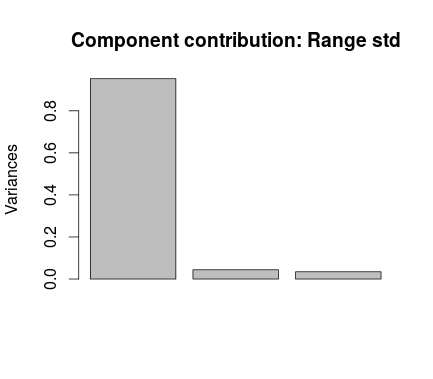
\includegraphics[width=\linewidth]{images/singular_values_rangenrm}
	\end{minipage}
	\hfill
	\begin{minipage}[h]{0.49\linewidth}
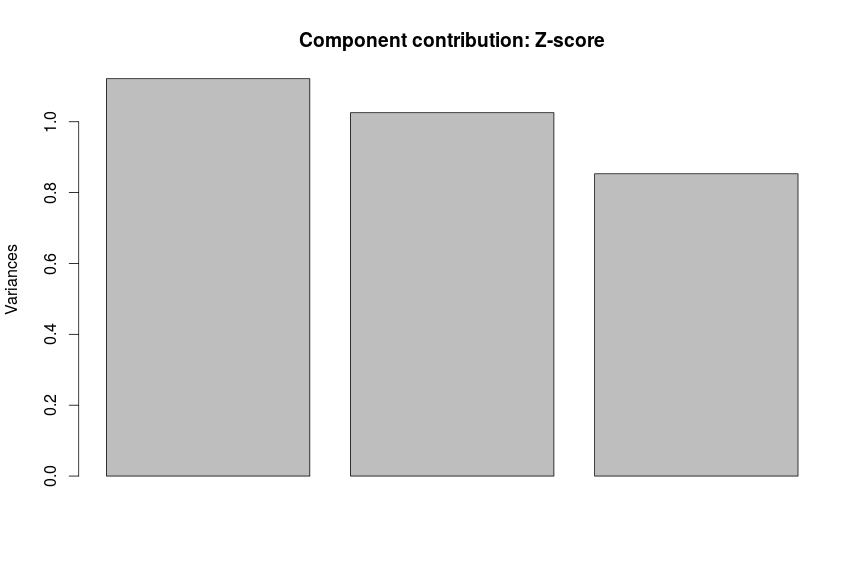
\includegraphics[width=\linewidth]{images/singular_values_zscore}
	\end{minipage}
	\vspace{-1cm}
	\caption{Summary contribution of first PC's to the data scatter according to different types of normalization techniques}
	\label{fig:data_scatter_contibution}
\end{figure} 


\subsection{Hidden factor}
As we have already mentioned, the hidden factor we have choosen is reader's attitude to an article. We assume that reader's attitude is "distirbuted" on the features that we have presented earlier. According to the model we have build this "distirbution" is approximated with vector of wights (also known as right singular vector which corresponds to the first principle component). These weighs are as follows: 
\begin{equation}
0.826968238, \qquad 0.008768395,\qquad 0.562180264
\end{equation}	

These numbers could be interpreted as the weighs of feature's values  which in turn sum up to the user's attitude. So the most influential features are from the most to least : \texttt{num\_imgs},  \texttt{shares}, \texttt{global\_sentiment\_polarity}. 
That also means, that the first principal factor is greater when the article contains more images and when the article has been sufficiently shared in various social media. 

Also, it is clear that impact of  \texttt{global\_sentiment\_polarity} on the principal component is negligible.  


Here we should point out, that the whole analisys of hidden factor and the corresponding coefficients is based on the initial, noncentered data. Any type of standardization could potentially invalidate any conclusion which could be made on such data. That is because of scaling effect and negativity values being multiplied with negative weights. 

That interesting fact was explained in \cite{CCODA_Mirkin}, and we based our homework on top of this fact,  which is discussed there in great detail.

The last step is not very interesting: we  should scale the resulted hidden variable values (which are the inner product of article's features and the weights vector) so as they form up the whole scale ranging from zero up to 100. 
The details of such a rescaling of hidden values  could be found in code snippet attached and is no of particular interest for us.






